
\normalsize

\section{Formal Definitions}

In this section, we formally define HAT transactional semantics. Our
formalism is based off of that of Adya~\cite{adya}. For the reader
familiar with his formalism, this is a mostly-straightforward exercise
combining transactional models with distributed systems
semantics. While the novel aspects of this work largely pertain
to \textit{using} these definitions (e.g., in Section~\ref{sec:hats}),
we believe it is instructive to accompany them by appropriate
definitions to both eliminate any ambiguity in prose and for the
enjoyment of more theoretically-inclined readers.

\subsection{Model}

Here, we briefly describe our database model. It is, with the
exception of sessions, identical to that of Adya~\cite{adya}. We omit
a full duplication of his formalism here but highlight several salient
criteria. We refer the interested reader to Adya's Ph.D. thesis,
Section 3.1 (pp. 33--43).

Users submit transactions to a database system that contains multiple
versions of sets of objects. Each transaction is composed of writes,
which create new versions of an object, and reads, which return a
written version or the initial version of the object. A transaction's
last operation is either \texttt{commit} or \texttt{abort}, and there
is exactly one invocation of either these two operations per
transaction. Transactions can either read individual items or read
based on predicates, or logical ranges of data items.

\begin{definition}[Version set of a predicate-based operation]
When a transaction executes a read or write based on a predicate P,
the system selects a version for each tuple in P’s relations. The set
of selected versions is called the \textit{Version set} of this predicate-based
operation and is denoted by Vset(P).
\end{definition}

A history over transactions has two parts: a partial order of events
reflects the ordering of operations with respect to each transaction
and a (total) version order ($\ll$) on the committed versions of each
object.

As a departure from Adya's formalism, to capture the use of session
guarantees, we allow transactions to be grouped into sessions. We
represent sessions as a partial ordering on committed transactions
such that each transaction in the history appears in at most one
session.

\subsection{Conflict and Serialization Graphs}

To reason about isolation anomalies, we use Adya's concept of a
conflict graph, which is composed of dependencies between
transaction. The definitions in this section are directly from Adya,
with two differences. First, we expand Adya's formalism to deal
with \textit{per-item} dependencies. Second, we define session
dependencies (Definition~\ref{def:sd1}).

\begin{definition}[Change the Matches of a Predicate-Based Read]
A transaction $T_i$ changes the matches
of a predicate-based read $r_j$(P:Vset(P)) if $T_i$ installs $x_i$, $x_h$
immediately precedes $x_i$ in the version order, and $x_h$ matches
P whereas $x_i$ does not or vice-versa. In this case, we also
say that $x_i$ changes the matches of the predicate-based read.
The above definition identifies $T_i$ to be a transaction where
a change occurs for the matched set of $r_j$ (P: Vset(P)).
\end{definition}

\begin{definition}[Directly Read-Depends{~\cite[Definition 2]{adya}}]
$T_j$ directly read-depends on transaction $T_i$ if it directly
item-read-depends or directly predicate-read-depends on $T_i$.
\end{definition}

\begin{definition}[Directly item-read-depends by $x$]
$T_j$ directly item-read-depends on transaction $T_i$ if $T_i$ installs some
  object version $x_i$ and $T_j$ reads $x_i$.
\end{definition}

\begin{definition}[Directly item-read-depends]
$T_j$ directly item-read-depends on transaction $T_i$ if $T_j$
  directly item-read-depends by $x$ on $T_i$ for some data item $x$.
\end{definition}

\begin{definition}[Directly predicate-read-depends by $P$]
Transaction $T_j$ directly predicate-read-depends by $P$ on
transaction $T_i$ if $T_j$ performs an operation $r_j$(P: Vset(P)),
$x_k$ $\in$ Vset(P), $i = k$ or $x_i \ll x_k$ , and $x_i$ changes the
matches of $r_j$ (P: Vset(P)).
\end{definition}

\begin{definition}[Directly predicate-read-depends]
$T_j$ directly predicate-read-depends on $T_i$ if $T_j$ directly
  predicate-read-depends by $P$ on $T_i$ for some predicate $P$.
\end{definition}

\begin{definition}[Directly Anti-Depends{~\cite[Definition 4]{adya}}]
Transaction $T_j$ directly anti-depends on transaction $T_i$ if it
directly item-anti-depends or directly predicate-anti-depends on
$T_i$.
\end{definition}

\begin{definition}[Directly item-anti-depends by $x$]
$T_j$ directly item-anti-depends by $x$ on transaction $T_i$ if $T_i$
  reads some object version $x_k$ and $T_j$ installs $x$'s next
  version (after $x_k$) in the version order. Note that the
  transaction that wrote the later version directly item-anti-depends
  on the transaction that read the earlier version.
\end{definition}

\begin{definition}[Directly item-anti-depends]
$T_j$ directly item-anti-depends on transaction $T_i$ if $T_j$
  directly item-anti-depends on transaction $T_i$.
\end{definition}

\begin{definition}[Directly predicate-anti-depends by $P$]
$T_j$ directly predicate-anti-depends by $P$ on transaction $T_i$ if
  $T_j$ overwrites an operation $r_i(P:$ Vset(P)). That is, if $T_j$
  installs a later version of some object that changes the matches of
  a predicate based read performed by $T_i$.
\end{definition}

\begin{definition}[Directly predicate-anti-depends by $P$]
$T_j$ directly predicate-anti-depends on transaction $T_i$ if $T_j$
  directly predicate anti-depends by $P$ on $T_i$ for some predicate
  $P$.
\end{definition}

\begin{definition}[Directly Write-Depends by $x$]
A transaction $T_j$ directly write-depends by $x$ on transaction $T_i$
if $T_i$ installs a version $x_i$ and $T_j$ installs $x$'s next
version (after $x_i$) in the version order.
\end{definition}

\begin{definition}[Directly Write-Depends{~\cite[Definition 5]{adya}}]
A transaction $T_j$ directly write-depends on transaction $T_i$ if
$T_i$ directly write-depends by $x$ on $T_j$ for some item $x$.
\end{definition}

\begin{definition}[Session-Depends]
\label{def:sd1}
A transaction $T_j$ session-depends on transaction $T_i$ if $T_i$ and
$T_j$ occur in the same session and $T_i$ precedes $T_j$ in the
session commit order.
\end{definition}

The dependencies for a history $H$ form a graph called its Directed
Serialization Graph ($DSG(H)$). If $T_j$ directly write-depends on
$T_i$ by $x$, we draw $T_i\overset{ww_x}\longrightarrow T_j$. If $T_j$
read-depends on $T_i$ by $x$, we draw
$T_i \overset{rw_x}\longrightarrow T_j$. If $T_j$ directly
anti-depends on transaction $T_j$ by $x$, we draw
$T_i \overset{wr_x}\DashedArrow T_j$. If $T_j$ session-depends on
$T_i$ in session $S$, we draw $T_i \overset{S}\longrightarrow
T_j$~\cite[Definition 8]{adya}.

We also consider the Unfolded Serialization Graph ($USG(H)$) that is a
variation of the $DSG$. The USG is specified for the transaction of
interest, $T_i$, and a history, $H$, and is denoted by $USG(H,
T_i)$. For the USG, we retain all nodes and edges of the $DSG$ except
for $T_i$ and the edges incident on it. Instead, we split the node for
$T_i$ into multiple nodes---one node for every read/write event in
$T_i$. The edges are now incident on the relevant event of $T_i$.

$USG(H, T_i)$ is obtained by transforming $DSG(H)$ as follows:.  For
each node $p$ ($p \neq T_i$) in $DSG(H)$, we add a node to
$USG(H,T_i)$. For each edge from node $p$ to node $q$ in $DSG(H)$,
where p and q are different from $T_i$, we draw a corresponding edge
in $USG(H,T_i)$. Now we add a node corresponding to every read and
write performed by $T_i$. Any edge that was incident on $T_i$ in the
$DSG$ is now incident on the relevant event of $T_i$ in the
$USG$. Finally, consecutive events in $T_i$ are connected
by \textit{order edges}, e.g., if an action (e.g., SQL statement)
reads object $y_j$ and immediately follows a write on object $x$ in
transaction $T_i$, we add an order-edge from $w_i(x_i)$ to
$r_i(y_j)$~\cite[Section 4.2.1]{adya}.

\subsection{Transactional Anomalies and Isolation Levels}

Following Adya, we define isolation levels according to
possible \textit{anomalies}--typically represented by cycles in the
serialization graphs. Definitions~\ref{def:n-ici}--\ref{def:lostupdate}
are not found in Adya but are found (albeit not in this formalism) in
Berenson et al.~\cite{ansicritique} and the literature on session
guarantees~\cite{sessionguarantees, vogels-defs}.

\begin{definition}[Write Cycles (G0)]
A history $H$ exhibits phenomenon G0 if $DSG(H)$ contains a directed
cycle consisting entirely of write-dependency edges.
\end{definition}

\begin{definition}[Read Uncommitted]
A system that provides Read Uncommitted isolation prohibits phenomenon G0.
\end{definition}

\begin{definition}[Aborted Reads (G1a)]
A history $H$ exhibits phenomenon G1a if it contains an aborted
transaction $T_1$ and a committed transaction $T_2$ such that $T_2$ has read
some object (maybe via a predicate) modified by $T_1$.
\end{definition}

\begin{definition}[Intermediate Reads (G1b)]
A history $H$ exhibits phenomenon G1b if it contains a committed
transaction $T_2$ that has read a version of object $x$ (maybe via a
predicate) written by transaction $T_1$ that was not $T_1$’s final
modification of $x$.
\end{definition}

\begin{definition}[Circular Information Flow (G1c)]
A history $H$ exhibits phenomenon G1c if $DSG(H)$ contains a directed
cycle consisting entirely of dependency edges.
\end{definition}

\begin{definition}[Read Committed]
A system that provides Read Committed isolation prohibits phenomenon G0, G1a, G1b, and G1c.
\end{definition}

\begin{definition}[Item-Many-Preceders (IMP)]
\label{def:imp}
A history $H$ exhibits phenomenon IMP if $DSG(H)$ contains a
transaction $T_i$ such that $T_i$ directly item-read-depends by $x$ on more
than one other transaction.
\end{definition}

\begin{figure}[H]
\begin{align*}
\small
T_1 &: w_x(1)\\
T_2 &: w_x(2)\\
T_3 &: r_x(1)~r_x(2)
\end{align*}
\caption{Example of \textit{IMP} anomaly.}
\label{fig:nici-history}
\end{figure}

\begin{figure}[H]
\centering
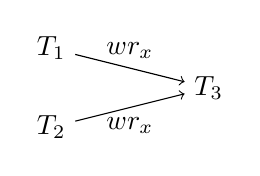
\begin{tikzpicture}[node distance=3cm]
\tikzstyle{tx}=[draw=none, fill=none]
\node[tx] (T1) at (0,0) {$T_1$};
\node[tx] (T2) at (0,-1) {$T_2$};
\node[tx] (T3) at (2,-.5) {$T_3$};

\draw[->] (T1) edge node[above]{$wr_x$} (T3);
\draw[->] (T2) edge node[below]{$wr_x$} (T3);
\end{tikzpicture}
\caption{DSG for Figure~\ref{fig:nici-history}.}
\label{fig:nici-dsg}
\end{figure}

\begin{definition}[Item Cut Isolation (I-CI)]
A system that provides Item Cut Isolation prohibits phenomenon IMP.
\end{definition}

\begin{definition}[Predicate-Many-Preceders (PMP)]
A history $H$ exhibits phenomenon PMP if, for all predicate-based
reads $r_i(P_i:Vset(P_i))$ and $r_j(P_j:Vset(P_j)$ in $T_k$ such that
the logical ranges of $P_i$ and $P_j$ overlap (call it $P_o$), the set
of transactions that change the matches of $P_o$ for $r_i$ and $r_j$
differ.
\end{definition}

\begin{definition}[Predicate Cut Isolation (P-CI)]
A system that provides Predicate Cut Isolation prohibits phenomenon PMP.
\end{definition}

\begin{definition}[Observed Transaction Vanishes (OTV)]
A history $H$ exhibits phenomenon OTV if $USG(H)$ contains a directed
cycle consisting of exactly one read-dependency edge by $x$ from $T_j$
to $T_i$ and a set of edges by $y$ containing at least one
anti-dependency edge from $T_i$ to $T_j$ and $T_j$'s read from $y$
precedes its read from $x$.
\end{definition}


\begin{figure}[H]
\begin{align*}
\small
T_1 &: w_x(1)~w_y(1)\\
T_2 &: w_x(2)~w_y(2)\\
T_3 &: r_x(2)~r_y(1)
\end{align*}
\caption{Example of \textit{OTV} anomaly.}
\label{fig:nta-history}
\end{figure}

\begin{figure}[H]
\centering
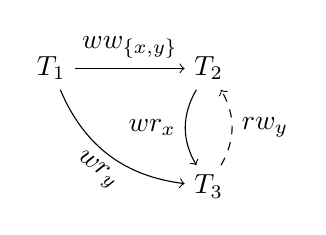
\begin{tikzpicture}[node distance=3cm]
\tikzstyle{tx}=[draw=none, fill=none]
\node[tx] (T1) at (0,0) {$T_1$};
\node[tx] (T2) at (2,0) {$T_2$};
\node[tx] (T3) at (2,-1.5) {$T_3$};

\draw[->] (T1) edge node[sloped, above]{$ww_{\{x, y\}}$} (T2);
\draw[->] (T1) edge [bend right] node[sloped, below]{$wr_y$} (T3);
\draw[->] (T2) edge [bend right] node[left]{$wr_x$} (T3);
\draw[dashed, ->] (T3) edge [bend right] node[right]{$rw_y$} (T2);
\end{tikzpicture}
\caption{DSG for Figure~\ref{fig:nta-history}.}
\label{fig:nta-dsg}
\end{figure}

\begin{definition}[Monotonic Atomic View (MAV)]
A system that provides Monotonic Atomic View isolation prohibits
phenomenon OTV in addition to providing Read Committed isolation.
\end{definition}

The following session guarantees are directly adapted from Terry et
al.'s original definitions~\cite{sessionguarantees}:

\begin{definition}[Non-monotonic Reads (N-MR)]
A history $H$ exhibits phenomenon N-MR if $DSG(H)$ contains a directed cycle
consisting of a transitive session-dependency between transactions
$T_j$ and $T_i$ with an anti-dependency edge by $i$ from $T_j$ and a
read-dependency edge by $i$ into $T_i$.
\end{definition}

\begin{definition}[Monotonic Reads (MR)]
A system provides Monotonic Reads if it prohibits phenomenon N-MR.
\end{definition}


\begin{figure}[H]
\begin{align*}
\small
T_1 &: w_x(1)\\
T_2 &: w_x(2)\\
T_3 &: r_x(2)\\
T_4 &: r_x(1)
\end{align*}
\caption{Example of \textit{N-MR} violation when $w_x(1) \ll w_x(2)$ and $T_4$ directly session-depends on $T_3$.}
\label{fig:nmr-history}
\end{figure}

\begin{figure}[H]
\centering
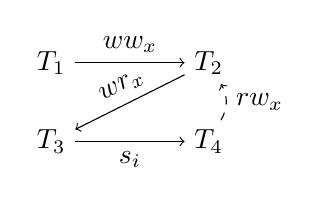
\begin{tikzpicture}[node distance=3cm]
\tikzstyle{tx}=[draw=none, fill=none]
\node[tx] (T1) at (0,0) {$T_1$};
\node[tx] (T2) at (2,0) {$T_2$};

\node[tx] (T3) at (0,-1) {$T_3$};
\node[tx] (T4) at (2,-1) {$T_4$};

\draw[->] (T1) edge node[above]{$ww_x$} (T2);
\draw[->] (T3) edge node[below]{$s_i$} (T4);

\draw[->] (T2) edge node[sloped, above]{$wr_x$} (T3);
%\draw[->] (T2) edge [bend right] node[left]{$wr_x$} (T4);
%\draw[->] (T1) edge [bend right]node[right]{$wr_x$} (T4);
\draw[dashed, ->] (T4) edge [bend right]node[right]{$rw_x$} (T2);
\end{tikzpicture}
\caption{DSG for Figure~\ref{fig:nmr-history}. $wr_x$ dependency from $T_1$ to $T_4$ omitted.} 
\label{fig:nmr-dsg}
\end{figure}

\begin{definition}[Non-monotonic Writes (N-MW)]
A history $H$ exhibits phenomenon N-MW if $DSG(H)$ contains a directed cycle
consisting of a transitive session-dependency between transactions
$T_j$ and $T_i$ and at least one write-dependency edge.
\end{definition}


\begin{figure}[H]
\begin{align*}
\small
T_1 &: w_x(1)\\
T_2 &: w_y(1)\\
T_3 &: r_y(1)~r_x(0)
\end{align*}
\caption{Example of \textit{N-MW} anomaly if $T_2$ directly session-depends on $T_1$.}
\label{fig:nmw-history}
\end{figure}

\begin{figure}[H]
\centering
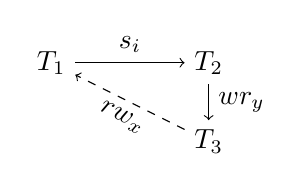
\begin{tikzpicture}[node distance=3cm]
\tikzstyle{tx}=[draw=none, fill=none]
\node[tx] (T1) at (0,0) {$T_1$};
\node[tx] (T2) at (2,0) {$T_2$};
\node[tx] (T3) at (2,-1) {$T_3$};

\draw[->] (T1) edge node[above]{$s_i$} (T2);
\draw[->] (T2) edge node[right]{$wr_y$} (T3);
\draw[->, dashed] (T3) edge node[below, sloped]{$rw_x$} (T1);
\end{tikzpicture}
\caption{DSG for Figure~\ref{fig:nmw-history}.}
\label{fig:nmw-dsg}
\end{figure}


\begin{definition}[Monotonic Writes (MW)]
A system provides Monotonic Writes if it prohibits phenomenon N-MW.
\end{definition}

\begin{definition}[Missing Read-Write Dependency (MRWD)]
A history $H$ exhibits phenomenon MRWD if, in $DSG(H)$, for all
committed transactions $T_1$, $T_2$, $T_3$ such that $T_2$
write-depends on $T_1$ and $T_3$ write-depends on $T_2$, $T_3$ does
not directly anti-depend on $T_1$.
\end{definition}


\begin{figure}[H]
\begin{align*}
\small
T_1 &: w_x(1)\\
T_2 &: r_x(1) w_y(1)\\
T_3 &: r_y(1)~r_x(0)
\end{align*}
\caption{Example of \textit{MRWD} anomaly.}
\label{fig:nwfr-history}
\end{figure}

\begin{figure}[H]
\centering
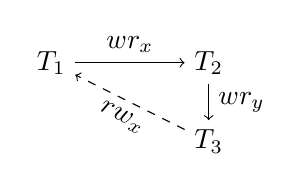
\begin{tikzpicture}[node distance=3cm]
\tikzstyle{tx}=[draw=none, fill=none]
\node[tx] (T1) at (0,0) {$T_1$};
\node[tx] (T2) at (2,0) {$T_2$};
\node[tx] (T3) at (2,-1) {$T_3$};

\draw[->] (T1) edge node[above]{$wr_x$} (T2);
\draw[->] (T2) edge node[right]{$wr_y$} (T3);
\draw[->, dashed] (T3) edge node[below, sloped]{$rw_x$} (T1);
\end{tikzpicture}
\caption{DSG for Figure~\ref{fig:nwfr-history}.}
\label{fig:nwfr-dsg}
\end{figure}

\begin{definition}[Writes Follow Reads (WFR)]
A system provides Writes Follow Reads if it prohibits phenomenon MWRD.
\end{definition}

\begin{definition}[Missing Your Writes (MYR)]
A history $H$ exhibits phenomenon MYR if $DSG(H)$ contains a directed cycle
consisting of a transitive session-dependency between transactions
$T_j$ and $T_i$, at least one anti-dependency edge, and the remainder
anti-dependency or write-dependency edges.
\end{definition}


\begin{figure}[H]
\begin{align*}
\small
T_1 &: w_x(1)\\
T_2 &: r_x(0)\\
\end{align*}
\caption{Example of \textit{MYR} anomaly if $T_2$ directly session-depends on $T_1$.}
\label{fig:nryw-history}
\end{figure}

\begin{figure}[H]
\centering
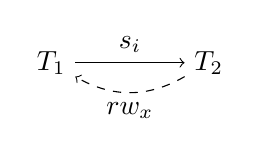
\begin{tikzpicture}[node distance=3cm]
\tikzstyle{tx}=[draw=none, fill=none]
\node[tx] (T1) at (0,0) {$T_1$};
\node[tx] (T2) at (2,0) {$T_2$};

\draw[->] (T1) edge node[above]{$s_i$} (T2);
\draw[dashed, ->] (T2) edge [bend left] node[below]{$rw_x$} (T1);
\end{tikzpicture}
\caption{DSG for Figure~\ref{fig:nwfr-history}.}
\label{fig:nryw-dsg}
\end{figure}

\begin{definition}[Read Your Writes (RYW)]
A system provides Read Your Writes if it prohibits phenomenon MYR.
\end{definition}

\begin{definition}[PRAM Consistency]
A system provides PRAM Consistency if it prohibits phenomenon N-MR,
N-MW, and MYR.
\end{definition}

\begin{definition}[Causal Consistency]
A system provides Causal Consistency if it provides PRAM Consistency
and prohibits phenomenon MWRD.
\end{definition}

\begin{definition}[Lost Update]
A history $H$ exhibits phenomenon Lost if $DSG(H)$ contains a directed
cycle having one or more item-antidependency edges and all edges are
by the same data item $x$.
\label{def:lostupdate}
\end{definition}

\begin{definition}[Write Skew (Adya G2-item)]
A history $H$ exhibits phenomenon Write Skew if $DSG(H)$ contains a directed
cycle having one or more item-antidependency edges.
\end{definition}

For Snapshot Isolation, we depart from Adya's recency-based definition
(see Adya Section 4.3). Nonetheless, implementations of this
definition will still be unavailable due to reliance of preventing
Lost Update.

\begin{definition}[Snapshot Isolation]
A system that provides Snapshot Isolation prevents phenomena G0, G1a,
G1b, G1c, PMP, OTV, and Lost Update.
\end{definition}

For Repeatable Read, we return to Adya.

\begin{definition}[Repeatable Read]
A system that provides Repeatable Read Isolation prohibits phenomena
G0, G1a, G1b, G1c, and Write Skew.
\end{definition}

For definitions of safe, regular, and linearizable register semantics,
we refer the reader to Herlihy's textbook~\cite{herlihy-art}.

\section{Monotonic Atomic View Isolation}

In this section, we provide additional information on our two-phase
algorithm for providing Monotonic Atomic View isolation. This section
is effectively a work-in-progress; we are actively investgating
alternative algorithms (particularly with respect to metadata
overheads) and stronger (but still HAT) semantics that complement the
techniques presented here. The interested reader (or would-be systems
implementer) should contact Peter Bailis for more details.

The below pseudocode describes a straightforward implementation of the
algorithm from Section~\ref{sec:ta}. Replicas maintain two sets of
data items: \texttt{pending} (which contains writes that are not yet
pending stable) and \texttt{good} (which contains writes that are
pending stable). Incoming writes are added to \texttt{pending} and
moved to \texttt{good} once they are stable. Stable pending
calculation is performed by counting the number of acknowledgments
(\texttt{acks}) of writes from other replicas, signifying their
receipt of the transaction's writes in their
own \texttt{pending}. Accordingly, the algorithm maintains the
invariant that the transactional siblings (or suitable replacements)
for every write in \texttt{good} are present on their respective
replicas. Clients use the RC algorithm from
Section~\ref{sec:isolation} and keep a map of data items to timestamps
(\texttt{required})---effectively a vector clock whose entries are
data items (not processes, as is standard).

\vspace{1em}\noindent\textbf{Example.} To illustrate this algorithm consider an execution of the following transactions:
\begin{align*}
\small\vspace{-1em}
T_1 &: w_x(1)~w_y(1)
\\T_2 &: r_x(1)~r_y(a)
\end{align*}
For MAV, the system must ensure that $a=1$. Consider a system with one
replica for each of $x$ and $y$ (denoted $R_x$ and $R_y$). Say client
$c_1$ executes $T_1$ and commits. The client chooses timestamp $10001$
(whereby the last $4$ digits are reserved for client ID to ensure
uniqueness) and sends values to $w_x(1)$ to $R_x$ and $R_y$ with
$tx\_keys = \{x,y\}$ and $timestamp=10001$. $R_x$ and $R_y$ place
their respective writes into their individual \texttt{pending} sets
and send acknowledgment for transaction timestamped $10001$ to the
other. Consider the case where $r_x$ has seen $r_y$'s acknowledgment
but not vice versa: $w_x(1)$ will be in \texttt{good} on $R_x$
but \texttt{pending} on $R_y$. Now, if another client $c_2$ executes
$T_2$ and reads $x$ from $R_x$, it will read $x=1$. $c_2$ will update
its \texttt{required} vector so that $\texttt{required}=\{x:10001,
y:10001\}$. When $c_2$ reads $y$ from $R_y$, it will specify
$ts=10001$ and $R_y$ will not find a suitable write
in \texttt{good}. $R_y$ will instead return $y=1$
from \texttt{pending}.

\vspace{1em}\noindent\textbf{Overheads.} MAV requires overhead both on client and server. First, clients must store a vector (\texttt{required}) for the duration of a transaction in order to determine what values to read. Second, each write contains metadata ($tx\_keys$) linear in the number of writes in the transaction. (Note that we could have stored a different timestamp with every write, but a single timestamp suffices and is more efficient) These overheads are modest for short transaction lengths but they increase value sizes on disk, in memory, and over the network. Third, on the server side, each client \textsc{put} incurs two back-ends \texttt{put}s: one into \texttt{pending} and \texttt{good}. If keeping a single value for \texttt{good}, the second \texttt{put} into \texttt{good} (as is the case with normal, single-valued eventually consistent operation) is really a \texttt{get} then a possible \texttt{put}: the server first checks if a higher-timestamped value has been written and, if not, it overwrites the current value. The \texttt{put} into \texttt{pending} is simpler: if message delivery is exactly-once, then \texttt{put}s can be made unconditionally.

\vspace{1em}\noindent\textbf{Optimizations.} The use of \texttt{pending} and \texttt{required} is effectively to
handle the above race condition, where some but not all replicas have
realized that a write is pending stable. With this in mind, there are
several optimizations we can perform:

If a replica serves a read from \texttt{pending}, it must mean one of
two things: either the write is stable pending or the writing client
for the write is requesting the data item (this second case does not
occur in the below pseudocode since own-writes are served out
of \texttt{write\_buffer}). In the former case, the replica can safely
install the write into \texttt{good}.

As we mention in Section~\ref{sec:ta}, the size of \texttt{good} can
be limited to a single item. Recall that any item can be served
from \texttt{good} as long as its timestamp is greater than the
required timestamp. Accordingly, if replicas store multiple writes
in \texttt{good}, any time they can serve a write from \texttt{good},
the highest-timestamped write is always a valid response candidate
(and, indeed, returning the highest-timestamped write provides the
best visibility). Note, however, that serving a higher-than-requested
timestamp from \texttt{pending} is dangerous: doing so might mean
returning a write that is not pending stable and, via appropriate
unfortunate partition behavior, force a client to stall while an
available replica waits for the write to arrive in \texttt{pending}.

The below pseudocode implements a push-based acknowledgment scheme: replicas
eagerly notify other replicas about \texttt{pending} writes. This need
not be the case and, indeed, it is wasteful: if a write
in \texttt{pending} has lower timestamp than the highest timestamped
write in \texttt{good}, it can safely be discarded. Especially for
data items with high temporal locality or data stores that are
replicated over WAN, this \texttt{pending} invalidation may be a
frequent event. Instead, replicas can periodically poll other replicas
for acknowledgments (i.e., asking for either a match
in \texttt{pending} or a higher timestamp in \texttt{good}); this
reduces both network utilization and, in the case of
durable \texttt{pending} and \texttt{good} sets, disk utilization.

There are ample opportunities for batching of pending and good
acknowledgments. Batching is easier in a push-based acknowledgment
scheme, as pull-based acknowledgments may require invalidation to
actually reduce network transfers. Moreover, if a replica is
responsible for several writes within a transaction, \textrm{notify}
messages can be coalesced. We have also observed that batching
multiple background operations together (particularly for
anti-entropy) allows for more efficient compression---especially
important in network-constrained environments.

\vspace{1em}\noindent\textbf{Implementation note.} Our implementation from Section~\ref{sec:evaluation} implements the below pseudocode, with batching between \textrm{notify} operations and a single-item \texttt{good}. We have not yet investigated the efficiency of a pull-based approach (mostly due to our choice of RPC library, which unfortunately does not currently handle multiple outstanding requests per socket). We have also not experimentally determined the visibility effect of the side-channel pending stable notifications as in the first optimization.

\begin{algorithm}[t!]
\newcommand{\myindent}{\hspace{-1em}}
\begin{addmargin}[-1em]{0em}% 1em left, 2em right

\begin{algorithmic}
\caption*{\textbf{Algorithm} HAT Read Atomic Isolation}\vspace{.5em}
\State{\textit{\textbf{Shared Data Types}}\\\vspace{.5em}
\texttt{timestamp}: unique, per transaction identifier\\
$\texttt{write}:[\texttt{key:}k, \texttt{value}:v, \texttt{timestamp}:ts, \texttt{set<key>}:sibs]$\\\hrulefill}\vspace{.5em}

  \State{\textbf{\textit{Server-side Data Structures and Methods}\\\vspace{.5em}
$\texttt{set<write>:pending}$\\
$\texttt{set<write>:good}$\\
$\texttt{map<timestamp, int>:acks}$}}\\

\Procedure{put}{\texttt{write}:$w$}
  \State \texttt{pending}.add($w$)
  \For{key $k_t \in w.sibs$}
  \State \{all replicas for $sib$\}.notify($w.ts$)
  \EndFor
  
  \State \textit{asynchronously send $w$ to other replicas via anti-entropy}
  \State \Return

  \EndProcedure\vspace{.5em}

  \Procedure{notify}{\texttt{timestamp}:$ts$}
  \State \texttt{acks}.get($ts$).increment()
  \If{all \texttt{acks} received for all replicas for $ts$'s $sibs$}
  \State \texttt{good}.add($w$)
  \State \texttt{pending}.remove($w$)  
  \EndIf  
  \EndProcedure\vspace{.5em}

  \Procedure{get}{\texttt{key}:$k$, \texttt{timestamp}:$ts_{required}$}
  \If{$ts_{required} = \bot$}
  \State \Return $w \in \texttt{good}$ s.t. $w.key = key$ with highest timestamp
  \ElsIf{$\exists~w \in \texttt{good}$ s.t. $w.key = key, w.ts \geq ts_{required}$}
  \State \Return $w$
  \Else
  \State \Return $w \in \texttt{pending}$ s.t. $w.key = key,  w.ts = ts_{required}$
  \EndIf
  \EndProcedure\\\vspace{-.5em}\hrulefill\vspace{.25em}

  \State{\textbf{\textit{Client-side Data Structures and Methods}\\\vspace{.5em}
$\texttt{int:cur\_txn}$\\
$\texttt{map<key, value>:write\_buffer}$\\
$\texttt{map<key, timestamp>:required}$}}\\


\Procedure{begin\_transaction}{}
  \State \texttt{cur\_txn} = \textit{new txn ID} \commentt{// (e.g., clientID+logicalClock)}
  \EndProcedure\vspace{.5em}

\Procedure{put}{\texttt{key:$k$}, \texttt{value:$v$}}
  \State \texttt{write\_buffer}.put($k$, $v$)
\EndProcedure\vspace{.5em}

\Procedure{get}{\texttt{key:$k$}}
  \If {$k \in \texttt{write\_buffer}$}
  \State \Return \texttt{write\_buffer}.get($k$) \commentt{// if we want per-TxN RYW}
  \EndIf

  \State $w\_{ret}$ = (available replica for $k$).get($k$, \texttt{required}.get($k$))
  \For {$(tx_{key} \in w_{ret}.sibs$}
  \If {$w_{ret}.ts > \texttt{required}.get(tx_{key})$}
  \State $\texttt{required}$.put$(tx_{key}, w_{ret}.ts)$
  \EndIf
  \EndFor

  \State \Return $w\_{ret}.value$
\EndProcedure\vspace{.5em}


\Procedure{commit}{}
 \For{$(tx_{key}, v) \in \texttt{write\_buffer}$}
 \State $r$ = (available replica for $tx_{key}$)
 \State $r$.put($[tx_{key}, v, \texttt{cur\_txn}, \texttt{write\_buffer}.keys()]$)
 \EndFor
  \State \textsc{cleanup()}
\EndProcedure\vspace{.5em}


\Procedure{abort}{}
  \State \textsc{cleanup()}
\EndProcedure\vspace{.5em}


\Procedure{cleanup}{}
  \State \texttt{write\_buffer}.clear()
  \State \texttt{required\_map}.clear()
\EndProcedure\vspace{.5em}


\end{algorithmic}
\end{addmargin}
\end{algorithm}
